\documentclass{exam}
\usepackage{mainExam}

\title{Évaluation de cours :\\ tableaux de variations}
\author{Seconde 9}
\date{28 Mars 2025}

\begin{document}
%Version 1
\maketitle
\begin{questions}
\question Dresser le tableau de variations des fonctions $f$ définies sur $[-5;5]$ dont les courbes représentatives sont données ci-dessous :
\begin{parts}
\begin{minipage}{0.45\textwidth}
\part\hfill

\begin{center}
\begin{tikzpicture}[scale=0.5]
\repereclassique{-5.25}{-5.25}{5.25}{5.25}{1};
\draw (-5,1.5) parabola[bend at end] (-2,4);
\draw (-2,4) parabola bend (1,-3) (5,0);
\draw (-5,1.5) node {$\bullet$};
\draw (5,0) node {$\bullet$};
\end{tikzpicture}

\vspace*{0.5cm}
\begin{tikzpicture}
\tkzTabInit[espcl=2]{$x$ / 1, Variation de $f$ / 2}{$-5$,,$5$};
\end{tikzpicture}
\end{center}
\part\hfill

\begin{center}
\begin{tikzpicture}[scale=0.5]
\repereclassique{-5.25}{-5.25}{5.25}{5.25}{1};
\draw (-5,-4) parabola bend (0,-1) (5,-2);
\draw (-5,-4) node {$\bullet$};
\draw (5,-2) node {$\bullet$};
\end{tikzpicture}

\vspace*{0.5cm}
\begin{tikzpicture}
\tkzTabInit[espcl=2]{$x$ / 1, Variation de $f$ / 2}{$-5$,,$5$};
\end{tikzpicture}
\end{center}
\end{minipage}
\hfill\vline\hfill
\begin{minipage}{0.45\textwidth}
\part\hfill

\begin{center}
\begin{tikzpicture}[scale=0.5]
\repereclassique{-5.25}{-5.25}{5.25}{5.25}{1};
\draw (-5,-1) -- (-4,-0.5) -- (-2,2) -- (0,2.5) -- (2.2, 4) -- (5,5);
\draw (-5,-1) node {$\bullet$};
\draw (5,5) node {$\bullet$};
\end{tikzpicture}

\vspace*{0.5cm}
\begin{tikzpicture}
\tkzTabInit[espcl=2]{$x$ / 1, Variation de $f$ / 2}{$-5$,,$5$};
\end{tikzpicture}
\end{center}

\part\hfill

\begin{center}
\begin{tikzpicture}[scale=0.5]
\repereclassique{-5.25}{-5.25}{5.25}{5.25}{1};
\draw (-5,-4) parabola bend (-2.5,3) (-2,2);
\draw (-2,2) parabola[bend at end] (0,-1);
\draw (0,-1) parabola (2,2);
\draw (2,2) -- (5,0);
\draw (-5,-4) node {$\bullet$};
\draw (5,0) node {$\bullet$};
\end{tikzpicture}

\vspace*{0.5cm}
\begin{tikzpicture}
\tkzTabInit[espcl=2]{$x$ / 1, Variation de $f$ / 2}{$-5$,,$5$};
\end{tikzpicture}
\end{center}
\end{minipage}
\end{parts}
\end{questions}
\newpage
%Version 2
\maketitle
\begin{questions}
\question Dresser le tableau de variations des fonctions $f$ définies sur $[-5;5]$ dont les courbes représentatives sont données ci-dessous :
\begin{parts}
\begin{minipage}{0.45\textwidth}
\part\hfill

\begin{center}
\begin{tikzpicture}[scale=0.5]
\repereclassique{-5.25}{-5.25}{5.25}{5.25}{1};
\draw (-5,4) -- (1,2) -- (3,3) -- (5,-1);
\draw (-5,4) node {$\bullet$};
\draw (5,-1) node {$\bullet$};
\end{tikzpicture}

\vspace*{0.5cm}
\begin{tikzpicture}
\tkzTabInit[espcl=2]{$x$ / 1, Variation de $f$ / 2}{$-5$,,$5$};
\end{tikzpicture}
\end{center}
\part\hfill

\begin{center}
\begin{tikzpicture}[scale=0.5]
\repereclassique{-5.25}{-5.25}{5.25}{5.25}{1};
\draw (-5,2) parabola bend (-1,-3) (5,3.5);
\draw (-5,2) node {$\bullet$};
\draw (5,3.5) node {$\bullet$};
\end{tikzpicture}

\vspace*{0.5cm}
\begin{tikzpicture}
\tkzTabInit[espcl=2]{$x$ / 1, Variation de $f$ / 2}{$-5$,,$5$};
\end{tikzpicture}
\end{center}
\end{minipage}
\hfill\vline\hfill
\begin{minipage}{0.45\textwidth}
\part\hfill

\begin{center}
\begin{tikzpicture}[scale=0.5]
\repereclassique{-5.25}{-5.25}{5.25}{5.25}{1};
\draw (-5,1) parabola[bend at end] (-2,0);
\draw (-2,0) parabola[bend at end] (0,-2);
\draw (0,-2) parabola[bend at end] (3,-3);
\draw (3,-3) parabola[bend at end] (5,-4);
\draw (-5,1) node {$\bullet$};
\draw (5,-4) node {$\bullet$};
\end{tikzpicture}

\vspace*{0.5cm}
\begin{tikzpicture}
\tkzTabInit[espcl=2]{$x$ / 1, Variation de $f$ / 2}{$-5$,,$5$};
\end{tikzpicture}
\end{center}

\part\hfill

\begin{center}
\begin{tikzpicture}[scale=0.5]
\repereclassique{-5.25}{-5.25}{5.25}{5.25}{1};
\draw (-5,4) parabola bend (-2.5,-3) (-2,-2);
\draw (-2,-2) parabola[bend at end] (0,1);
\draw (0,1) parabola (2,-2);
\draw (2,-2) -- (5,0);
\draw (-5,4) node {$\bullet$};
\draw (5,0) node {$\bullet$};
\end{tikzpicture}

\vspace*{0.5cm}
\begin{tikzpicture}
\tkzTabInit[espcl=2]{$x$ / 1, Variation de $f$ / 2}{$-5$,,$5$};
\end{tikzpicture}
\end{center}
\end{minipage}
\end{parts}
\end{questions}
\newpage
%Version 3
\maketitle
\begin{questions}
\question Dresser le tableau de variations des fonctions $f$ définies sur $[-5;5]$ dont les courbes représentatives sont données ci-dessous :
\begin{parts}
\begin{minipage}{0.45\textwidth}
\part\hfill

\begin{center}
\begin{tikzpicture}[scale=0.5]
\repereclassique{-5.25}{-5.25}{5.25}{5.25}{1};
\draw (-5,-4) parabola bend (0,-1) (5,-2);
\draw (-5,-4) node {$\bullet$};
\draw (5,-2) node {$\bullet$};
\end{tikzpicture}

\vspace*{0.5cm}
\begin{tikzpicture}
\tkzTabInit[espcl=2]{$x$ / 1, Variation de $f$ / 2}{$-5$,,$5$};
\end{tikzpicture}
\end{center}

\part\hfill

\begin{center}
\begin{tikzpicture}[scale=0.5]
\repereclassique{-5.25}{-5.25}{5.25}{5.25}{1};
\draw (-5,-4) parabola bend (-2.5,3) (-2,2);
\draw (-2,2) parabola[bend at end] (0,-1);
\draw (0,-1) parabola (2,2);
\draw (2,2) -- (5,0);
\draw (-5,-4) node {$\bullet$};
\draw (5,0) node {$\bullet$};
\end{tikzpicture}

\vspace*{0.5cm}
\begin{tikzpicture}
\tkzTabInit[espcl=2]{$x$ / 1, Variation de $f$ / 2}{$-5$,,$5$};
\end{tikzpicture}
\end{center}

\end{minipage}
\hfill\vline\hfill
\begin{minipage}{0.45\textwidth}
\part\hfill

\begin{center}
\begin{tikzpicture}[scale=0.5]
\repereclassique{-5.25}{-5.25}{5.25}{5.25}{1};
\draw (-5,-1) -- (-4,-0.5) -- (-2,2) -- (0,2.5) -- (2.2, 4) -- (5,5);
\draw (-5,-1) node {$\bullet$};
\draw (5,5) node {$\bullet$};
\end{tikzpicture}

\vspace*{0.5cm}
\begin{tikzpicture}
\tkzTabInit[espcl=2]{$x$ / 1, Variation de $f$ / 2}{$-5$,,$5$};
\end{tikzpicture}
\end{center}

\part\hfill

\begin{center}
\begin{tikzpicture}[scale=0.5]
\repereclassique{-5.25}{-5.25}{5.25}{5.25}{1};
\draw (-5,1.5) parabola[bend at end] (-2,4);
\draw (-2,4) parabola bend (1,-3) (5,0);
\draw (-5,1.5) node {$\bullet$};
\draw (5,0) node {$\bullet$};
\end{tikzpicture}

\vspace*{0.5cm}
\begin{tikzpicture}
\tkzTabInit[espcl=2]{$x$ / 1, Variation de $f$ / 2}{$-5$,,$5$};
\end{tikzpicture}
\end{center}
\end{minipage}
\end{parts}
\end{questions}
\newpage

\end{document}
